\hiddenchapter{설계 산출물}
\ChapterTitle[\thechapter]{설계 산출물}
%%% See Preamble for an explanation of both of these %%%

\setcounter {section}{0}

\hiddensection{업무 분석: Application Modeling}
\SectionTitle{\thesection}{업무 분석: Application Modeling}

% \hiddensubsection{설계 표준}
\subsection{설계 표준}

\hspace{3em} 용어정리

\begin{longtable}
    {
        |>{\centering\hspace{0pt}}m{0.300\linewidth}
        |>{\centering\hspace{0pt}}m{0.300\linewidth}
        |>{\hspace{0pt}}m{0.200\linewidth}|
    } 
    \hline
    \rowcolor{aliceblue} \textbf{한글명} & \textbf{영어명} & \multicolumn{1}{c|}{\textbf{비고}}\\ 
    \hline
    등록 & Add & \\ 
    \hline
    목록 & List & \\ 
    \hline
    삭제 & Delete & \\ 
    \hline
    검색 & Search & \\ 
    \hline
    선택 & Select & \\ 
    \hline
    로그인 & Login & \\ 
    \hline
    로그아웃 & Logout & \\ 
    \hline
    수정 & Update & \\ 
    \hline
    조회 & Get & \\ 
    \hline
    인증 & Check & \\ 
    \hline
    완료 & Success & \\ 
    \hline
    신고 & Report & \\  
    \hline
    상태 & Status & \\ 
    \hline
    공개/비공개 & isPublic & \\ 
    \hline
    주소 & address & \\ 
    \hline
\end{longtable}

\hspace{2em} 소스파일

\hspace{3em} \small{JSP 파일 (Webcontent)}

\hspace{4em} \footnotesize{회원관리(User)}

\begin{longtable}
    {
        |>{\centering\hspace{0pt}}m{0.300\linewidth}
        |>{\centering\hspace{0pt}}m{0.300\linewidth}
        |>{\hspace{0pt}}m{0.200\linewidth}|
    } 
    \hline
    \rowcolor{aliceblue} \textbf{UI 구분} & \textbf{파일명} & \multicolumn{1}{c|}{\textbf{비고}}\\ 
    \hline
    로그인 & login.jsp &  \\ 
    \hline
    회원가입 & addUser.jsp &  \\ 
    \hline
    정지유저 로그인 불가 & ban.jsp &  \\ 
    \hline
    회원가입 완료 & successJoin.jsp &  \\ 
    \hline
    개인프로필 조회 & getMyUser.jsp &  \\ 
    \hline
    타인프로필조회 & getUser.jsp &  \\ 
    \hline
    개인프로필 수정 & updateUser.jsp &  \\ 
    \hline
    회원 목록 조회 & listUser.jsp &  \\ 
    \hline
    계정 신고 화면 & addUser.jsp &  \\ 
    \hline
    통합검색 유저 & listTotalUser.jsp &  \\ 
    \hline
    블랙리스트 목록 [Blacklist] & listBlacklist.jsp &  \\ 
    \hline
    블랙리스트 상세조회 & getBlacklist.jsp &  \\ 
    \hline
    신고내역 & listReport.jsp &  \\ 
    \hline
\end{longtable}

\hspace{3em} \small{기록관리(Diary)}

\begin{longtable}
    {
        |>{\centering\hspace{0pt}}m{0.300\linewidth}
        |>{\centering\hspace{0pt}}m{0.300\linewidth}
        |>{\hspace{0pt}}m{0.200\linewidth}|
    } 
    \hline
    \rowcolor{aliceblue} \textbf{UI 구분} & \textbf{파일명} & \multicolumn{1}{c|}{\textbf{비고}}\\ 
    \hline
    지도에서 장소 선택 & selectMap.jsp &  \\ 
    \hline
    기록 작성 & addDiary.jsp &  \\ 
    \hline
    내 기록 상세조회 & getMyDiary.jsp &  \\ 
    \hline
    타 회원 공개기록 상세조회 & getDiary.jsp &  \\ 
    \hline
    여행 타임라인 & timeline.jsp &  \\ 
    \hline
    내 기록 지도 & getDiaryMap.jsp &  \\ 
    \hline
    내 기록 목록 & listDiary.jsp &  \\ 
    \hline
    기록 휴지통 & diaryBin.jsp &  \\ 
    \hline
    기록 좌측 툴바 & leftbar.jsp &  \\ 
    \hline
    기록 그룹 목록 & listDiaryGroup.jsp &  \\ 
    \hline
    그룹별 기록 목록 & listDiaryByGroup.jsp &  \\ 
    \hline
    기록 그룹 선택 & selectDiaryGroup.jsp &  \\ 
    \hline
    기록 그룹명 수정 & updateGroupName.jsp &  \\ 
    \hline
    기록 수정 & updateDiary.jsp &  \\
    \hline
\end{longtable}

\hspace{3em} \small{후기관리(Review)}

\begin{longtable}
    {
        |>{\centering\hspace{0pt}}m{0.300\linewidth}
        |>{\centering\hspace{0pt}}m{0.300\linewidth}
        |>{\hspace{0pt}}m{0.200\linewidth}|
    } 
    \hline
    \rowcolor{aliceblue} \textbf{UI 구분} & \textbf{파일명} & \multicolumn{1}{c|}{\textbf{비고}}\\ 
    \hline
    후기작성 & addReview.jsp &  \\ 
    \hline
    후기조회 & getReview.jsp &  \\ 
    \hline
    후기수정 & updateReview.jsp &  \\ 
    \hline
    후기목록 & listReview.jsp &  \\ 
    \hline
    통합 검색 & listTotalReview.jsp &  \\
    \hline
\end{longtable}

\hspace{3em} \small{사진관리(Photo)}

\begin{longtable}
    {
        |>{\centering\hspace{0pt}}m{0.300\linewidth}
        |>{\centering\hspace{0pt}}m{0.300\linewidth}
        |>{\hspace{0pt}}m{0.200\linewidth}|
    } 
    \hline
    \rowcolor{aliceblue} \textbf{UI 구분} & \textbf{파일명} & \multicolumn{1}{c|}{\textbf{비고}}\\ 
    \hline
    목록으로 보기 & listPhoto.jsp &  \\ 
    \hline
    앨범 & album.jsp &  \\ 
    \hline
    사진 휴지통 & photoBin.jsp &  \\ 
    \hline
    앨범이동 & selectPhotoGroup.jsp &  \\ 
    \hline
    앨범명 수정 & updateGroupName.jsp &  \\
    \hline
\end{longtable}

\hspace{3em} \small{게시글 관리(Post)}

\begin{longtable}
    {
        |>{\centering\hspace{0pt}}m{0.300\linewidth}
        |>{\centering\hspace{0pt}}m{0.300\linewidth}
        |>{\hspace{0pt}}m{0.200\linewidth}|
    }
    \hline
    \rowcolor{aliceblue} \textbf{UI 구분} & \textbf{파일명} & \multicolumn{1}{c|}{\textbf{비고}}\\ 
    \hline
    내 게시글 상세조회 & getMyPost.jsp &  \\ 
    \hline
    타 회원 게시글 상세조회 & getPost.jsp &  \\ 
    \hline
    게시글 작성 & addPost.jsp &  \\ 
    \hline
    게시글 수정 & updatePost.jsp &  \\ 
    \hline
    내 댓글 목록 [comment] & listMyComment.jsp &  \\ 
    \hline
    사이드바 & leftbar.jsp &  \\ 
    \hline
    내 게시글 목록 & listPostBynickname.jsp &  \\
    \hline
\end{longtable}

\hspace{3em} \small{메인, 구독 관리(Subscribe), 북마크(Bookmark)}

\begin{longtable}
    {
        |>{\centering\hspace{0pt}}m{0.300\linewidth}
        |>{\centering\hspace{0pt}}m{0.300\linewidth}
        |>{\hspace{0pt}}m{0.200\linewidth}|
    }
    \hline
    \rowcolor{aliceblue} \textbf{UI 구분} & \textbf{파일명} & \multicolumn{1}{c|}{\textbf{비고}}\\ 
    \hline
    메인 화면 & main.jsp &  \\ 
    \hline
    툴바 & toolbar.jsp &  \\ 
    \hline
    구독자 목록 + 구독자가 쓴 기록 목록  & listSubscribe.jsp &  \\ 
    \hline
    북마크 목록 & listBookmark.jsp &  \\ 
    \hline
\end{longtable}

\hspace{3em} \small{메인, 구독 관리(Subscribe), 북마크(Bookmark)}

\begin{longtable}
    {
        |>{\centering\hspace{0pt}}m{0.300\linewidth}
        |>{\centering\hspace{0pt}}m{0.300\linewidth}
        |>{\hspace{0pt}}m{0.200\linewidth}|
    }
    \hline
    \rowcolor{aliceblue} \textbf{UI 구분} & \textbf{파일명} & \multicolumn{1}{c|}{\textbf{비고}}\\ 
    \hline
    메인 화면 & main.jsp &  \\ 
    \hline
    툴바 & toolbar.jsp &  \\ 
    \hline
    구독자 목록 + 구독자가 쓴 기록 목록  & listSubscribe.jsp &  \\ 
    \hline
    북마크 목록 & listBookmark.jsp &  \\ 
    \hline
\end{longtable}








\newpage

\hiddensubsection{Class Diagram \& VOPC \small(View Of Participating Class) \normalsize{Diagram}}
\begin{longtable}
    {
        |>{\centering\hspace{0pt}}m{0.300\linewidth}
        >{\raggedleft\hspace{0pt}}m{0.300\linewidth}
        >{\hspace{0pt}}m{0.200\linewidth}|
    } 
    \hline
    \multicolumn{3}{|c|}{\cellcolor{aliceblue}{}} \\
    \multicolumn{3}{|c|}{\cellcolor{aliceblue}{\Large\textbf{Class \& VOPC\normalsize{(View Of Participating Class)} \Large{Diagram}}}} \\
    \multicolumn{3}{|c|}{\cellcolor{aliceblue}{}} \\
    \hline
    \rowcolor{aliceblue} 
    {\normalsize{시스템 명: Travel Diary}}
    & {\normalsize{작성일: 2021년 2월 16일}}
    & \multicolumn{1}{r|}{\normalsize{작성자: 왕밤빵}} \\ \hline
    \multicolumn{3}{|c|}{\includegraphics[width=14.85cm]{./Figure/Design/Class_n_VOPC/User_ClassDiagram.pdf}} \\
    \hline
\end{longtable}
\normalsize
\newpage

\begin{longtable}
    {
        |>{\centering\hspace{0pt}}m{0.300\linewidth}
        >{\raggedleft\hspace{0pt}}m{0.300\linewidth}
        >{\hspace{0pt}}m{0.200\linewidth}|
    } 
    \hline
    \multicolumn{3}{|c|}{\cellcolor{aliceblue}{}} \\
    \multicolumn{3}{|c|}{\cellcolor{aliceblue}{\Large\textbf{Class \& VOPC\normalsize{(View Of Participating Class)} \Large{Diagram}}}} \\
    \multicolumn{3}{|c|}{\cellcolor{aliceblue}{}} \\
    \hline
    \rowcolor{aliceblue} 
    {\normalsize{시스템 명: Travel Diary}}
    & {\normalsize{작성일: 2021년 2월 16일}}
    & \multicolumn{1}{r|}{\normalsize{작성자: 왕밤빵}} \\ \hline
    \multicolumn{3}{|c|}{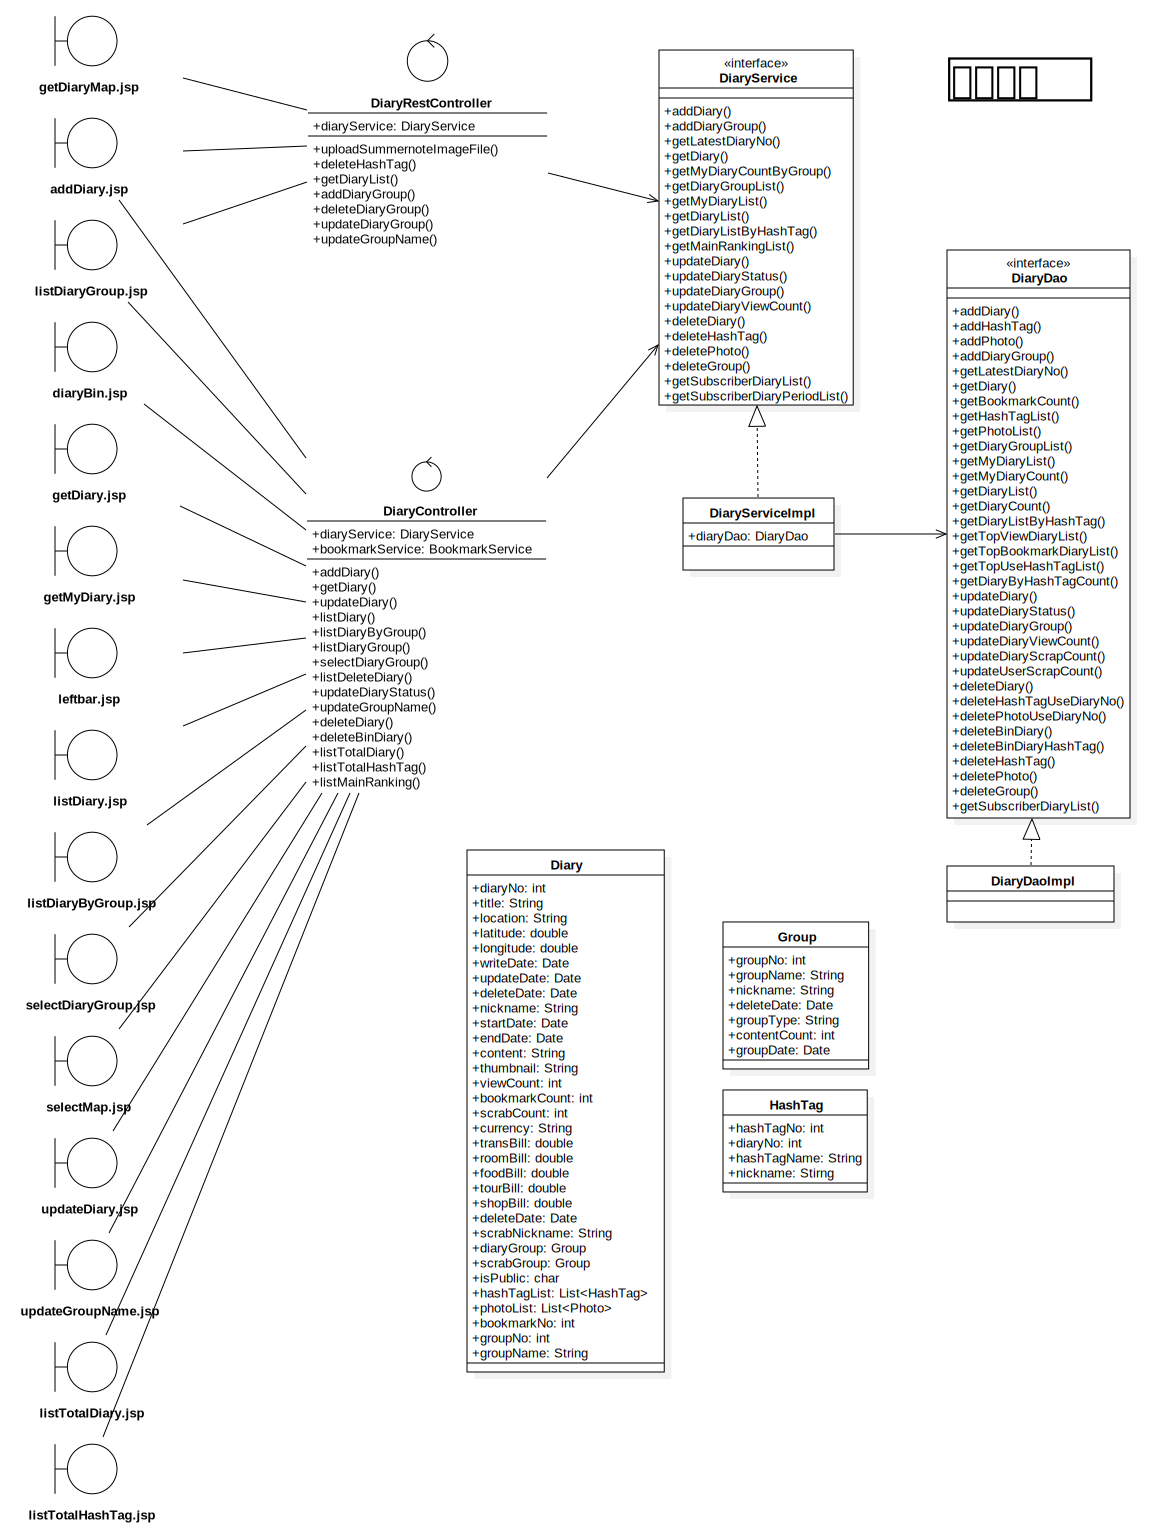
\includegraphics[width=16.00cm]{./Figure/Design/Class_n_VOPC/Diary_ClassDiagram.pdf}} \\
    \hline
\end{longtable}
\normalsize
\newpage

\begin{longtable}
    {
        |>{\centering\hspace{0pt}}m{0.300\linewidth}
        >{\raggedleft\hspace{0pt}}m{0.300\linewidth}
        >{\hspace{0pt}}m{0.200\linewidth}|
    } 
    \hline
    \multicolumn{3}{|c|}{\cellcolor{aliceblue}{}} \\
    \multicolumn{3}{|c|}{\cellcolor{aliceblue}{\Large\textbf{Class \& VOPC\normalsize{(View Of Participating Class)} \Large{Diagram}}}} \\
    \multicolumn{3}{|c|}{\cellcolor{aliceblue}{}} \\
    \hline
    \rowcolor{aliceblue} 
    {\normalsize{시스템 명: Travel Diary}}
    & {\normalsize{작성일: 2021년 2월 16일}}
    & \multicolumn{1}{r|}{\normalsize{작성자: 왕밤빵}} \\ \hline
    \multicolumn{3}{|c|}{\includegraphics[width=16.00cm]{./Figure/Design/Class_n_VOPC/Photo_ClassDiagram.pdf}} \\
    \hline
\end{longtable}
\normalsize
\newpage

\begin{longtable}
    {
        |>{\centering\hspace{0pt}}m{0.300\linewidth}
        >{\raggedleft\hspace{0pt}}m{0.300\linewidth}
        >{\hspace{0pt}}m{0.200\linewidth}|
    } 
    \hline
    \multicolumn{3}{|c|}{\cellcolor{aliceblue}{}} \\
    \multicolumn{3}{|c|}{\cellcolor{aliceblue}{\Large\textbf{Class \& VOPC\normalsize{(View Of Participating Class)} \Large{Diagram}}}} \\
    \multicolumn{3}{|c|}{\cellcolor{aliceblue}{}} \\
    \hline
    \rowcolor{aliceblue} 
    {\normalsize{시스템 명: Travel Diary}}
    & {\normalsize{작성일: 2021년 2월 16일}}
    & \multicolumn{1}{r|}{\normalsize{작성자: 왕밤빵}} \\ \hline
    \multicolumn{3}{|c|}{\includegraphics[width=16.00cm]{./Figure/Design/Class_n_VOPC/Post_ClassDiagram.pdf}} \\
    \hline
\end{longtable}
\normalsize
\newpage

\begin{longtable}
    {
        |>{\centering\hspace{0pt}}m{0.300\linewidth}
        >{\raggedleft\hspace{0pt}}m{0.300\linewidth}
        >{\hspace{0pt}}m{0.200\linewidth}|
    } 
    \hline
    \multicolumn{3}{|c|}{\cellcolor{aliceblue}{}} \\
    \multicolumn{3}{|c|}{\cellcolor{aliceblue}{\Large\textbf{Class \& VOPC\normalsize{(View Of Participating Class)} \Large{Diagram}}}} \\
    \multicolumn{3}{|c|}{\cellcolor{aliceblue}{}} \\
    \hline
    \rowcolor{aliceblue} 
    {\normalsize{시스템 명: Travel Diary}}
    & {\normalsize{작성일: 2021년 2월 16일}}
    & \multicolumn{1}{r|}{\normalsize{작성자: 왕밤빵}} \\ \hline
    \multicolumn{3}{|c|}{\includegraphics[width=16.00cm]{./Figure/Design/Class_n_VOPC/Bookmark_ClassDiagram.pdf}} \\
    \hline
\end{longtable}
\normalsize
\newpage

\begin{longtable}
    {
        |>{\centering\hspace{0pt}}m{0.300\linewidth}
        >{\raggedleft\hspace{0pt}}m{0.300\linewidth}
        >{\hspace{0pt}}m{0.200\linewidth}|
    } 
    \hline
    \multicolumn{3}{|c|}{\cellcolor{aliceblue}{}} \\
    \multicolumn{3}{|c|}{\cellcolor{aliceblue}{\Large\textbf{Class \& VOPC\normalsize{(View Of Participating Class)} \Large{Diagram}}}} \\
    \multicolumn{3}{|c|}{\cellcolor{aliceblue}{}} \\
    \hline
    \rowcolor{aliceblue} 
    {\normalsize{시스템 명: Travel Diary}}
    & {\normalsize{작성일: 2021년 2월 16일}}
    & \multicolumn{1}{r|}{\normalsize{작성자: 왕밤빵}} \\ \hline
    \multicolumn{3}{|c|}{\includegraphics[width=16.00cm]{./Figure/Design/Class_n_VOPC/Review_ClassDiagram.pdf}} \\
    \hline
\end{longtable}
\normalsize
\newpage

\begin{longtable}
    {
        |>{\centering\hspace{0pt}}m{0.300\linewidth}
        >{\raggedleft\hspace{0pt}}m{0.300\linewidth}
        >{\hspace{0pt}}m{0.200\linewidth}|
    } 
    \hline
    \multicolumn{3}{|c|}{\cellcolor{aliceblue}{}} \\
    \multicolumn{3}{|c|}{\cellcolor{aliceblue}{\Large\textbf{Class \& VOPC\normalsize{(View Of Participating Class)} \Large{Diagram}}}} \\
    \multicolumn{3}{|c|}{\cellcolor{aliceblue}{}} \\
    \hline
    \rowcolor{aliceblue} 
    {\normalsize{시스템 명: Travel Diary}}
    & {\normalsize{작성일: 2021년 2월 16일}}
    & \multicolumn{1}{r|}{\normalsize{작성자: 왕밤빵}} \\ \hline
    \multicolumn{3}{|c|}{\includegraphics[width=16.00cm]{./Figure/Design/Class_n_VOPC/Subscribe_ClassDiagram.pdf}} \\
    \hline
\end{longtable}
\normalsize
\newpage


\hiddensection{화면 분석}
\SectionTitle{\thesection}{화면 분석}



\newpage

\hiddensubsection{화면 정의서}
{\includegraphics[width=20cm]{./Figure/Analysis/Display/diary/diary_00.pdf} \\


\newpage

\hiddensection{데이터 분석(Physical)}
\SectionTitle{\thesection}{데이터 분석(Physical)}

\normalsize
\hiddensubsection{ERD{\small(Physical)}}

\begin{longtable}
    {
        |>{\centering\hspace{0pt}}m{0.300\linewidth}
        >{\raggedleft\hspace{0pt}}m{0.300\linewidth}
        >{\hspace{0pt}}m{0.200\linewidth}|
    } 
    \hline
    \multicolumn{3}{|c|}{\cellcolor{aliceblue}{}} \\
    \multicolumn{3}{|c|}{\cellcolor{aliceblue}{\Large\textbf{Entity Relationship Diagram\normalsize{(Physical)}}}} \\
    \multicolumn{3}{|c|}{\cellcolor{aliceblue}{}} \\
    \hline
    \rowcolor{aliceblue} 
    {\normalsize{시스템 명: Travel Diary}}
    & {\normalsize{작성일: 2021년 1월 13일}}
    & \multicolumn{1}{r|}{\normalsize{작성자: 왕밤빵}} \\ \hline
    \multicolumn{3}{|c|}{\includegraphics[width=15.75cm]{./Figure/Design/ERDDiagram(Physical).pdf}} \\
    \hline
\end{longtable}
\normalsize
\newpage



\hiddensubsection{테이블 목록}


\newpage



\hiddensubsection{테이블 정의서}


\newpage
